\chapter{Testen en Resultaten}%
\label{ch:testen}

\section{Doel van de testfase}
Het doel van deze testfase is het evalueren van de effectiviteit van de ontwikkelde prijsvergelijkingsapplicatie. De evaluatie focust op:
\begin{itemize}
    \item de correctheid van de selectie van de goedkoopste optie (met nadruk op \emph{prijs per eenheid}),
    \item de relevantie van de gevonden producten (kwaliteit van productmatching),
    \item de mate waarin het systeem manuele prijsvergelijking kan ondersteunen of vervangen,
    \item de robuustheid over verschillende productcategorieën (voeding en non-food).
\end{itemize}

De automatisch gegenereerde resultaten worden vergeleken met een manueel samengestelde referentiewinkelmand die fungeert als \emph{ground truth}. Hierbij wordt expliciet rekening gehouden met het feit dat manuele selectie vaak gestuurd wordt door totale prijs of promoties, terwijl de applicatie primair optimaliseert op prijs per eenheid.

\section{Methodologie}

\subsection{Referentiewinkelmand (manuele data)}
De referentiedata werd manueel verzameld door de auteur op de websites van de winkels (Albert Heijn, Colruyt en Carrefour), zoals een gemiddelde consument dit zou doen. Voor elk product werd:
\begin{itemize}
    \item het product afzonderlijk opgezocht,
    \item een representatieve match geselecteerd,
    \item indien beschikbaar de prijs per eenheid gebruikt,
    \item anders gesorteerd op laagste totale prijs en vervolgens manueel gecontroleerd op relevantie.
\end{itemize}

\subsection{Automatische data (applicatie)}
De applicatie verzamelt productinformatie via webscraping en rangschikt resultaten op basis van prijs per eenheid. Hiervoor wordt fuzzy matching toegepast om semantisch minder relevante matches (bv.\ dierenvoeding bij ``kip'' of schoonmaakproducten bij ``mandarijn'') lager te positioneren. Voor elk item in de winkelmand wordt de goedkoopste optie geselecteerd volgens het gekozen sorteercriterium.

\subsection{Testset}
De methoden werden toegepast op de volgende zeven winkelmanden:
\begin{enumerate}
    \item melk, boter, kip, brood
    \item bananen, ijs
    \item mandarijn, pesto, selderij, rigatoni
    \item pleister, rijst
    \item noedels, mayonaise, kaas
    \item wafel, pannenkoek, blauwe bessen
    \item maandverband, blush, toiletpapier
\end{enumerate}

\section{Resultaten}

\subsection{Vergelijking op basis van totale productprijs (``€/product'')}
In deze subsectie wordt per winkelmand de totale kost vergeleken tussen:
(i) manuele selectie per winkel en (ii) automatische selectie door de applicatie. 
Dit meet de praktische impact voor een gebruiker die één winkelmand wil samenstellen met minimale \emph{totale} uitgave.

\subsubsection{Winkelmand 1: melk, boter, kip en brood}
\begin{table}[H]
    \centering
    \begin{threeparttable}
        \caption{Winkelmand 1: totale productprijs (€/product)}
        \renewcommand{\arraystretch}{1.15}
        \begin{tabular}{lrrrrr}
            \toprule
            \textbf{Product} & \textbf{Colruyt} & \textbf{AH} & \textbf{Carrefour} & \textbf{App €/eh} & \textbf{App €/product} \\
            \midrule
            Melk  & 0.75 & 0.75 & 0.59 & 0.69 & 0.69 \\
            Boter & 2.09 & 1.59 & 0.99 & 22.80 & 22.80 \\
            Kip   & 4.19 & 3.49 & 2.30 & 18.19 & 18.19 \\
            Brood & 0.89 & 0.59 & 0.99 & 0.99 & 0.99 \\
            \midrule
            \textbf{Totaal} & \textbf{7.92} & \textbf{6.42} & \textbf{4.87} & \textbf{42.67} & \textbf{42.67} \\
            \bottomrule
        \end{tabular}
    \end{threeparttable}
    \label{tab:wm1_price}
\end{table}

\subsubsection{Winkelmand 2: bananen en ijs}
\begin{table}[H]
    \centering
    \begin{threeparttable}
        \caption{Winkelmand 2: totale productprijs (€/product)}
        \renewcommand{\arraystretch}{1.15}
        \begin{tabular}{lrrrrr}
            \toprule
            \textbf{Product} & \textbf{Colruyt} & \textbf{AH} & \textbf{Carrefour} & \textbf{App €/eh} & \textbf{App €/product} \\
            \midrule
            Bananen & 1.49 & 0.94 & 0.99 & 1.29 & 1.29 \\
            IJs     & 2.99 & 1.20 & 1.49 & 6.15 & 6.15 \\
            \midrule
            \textbf{Totaal} & \textbf{4.48} & \textbf{2.14} & \textbf{2.48} & \textbf{7.44} & \textbf{7.44} \\
            \bottomrule
        \end{tabular}
    \end{threeparttable}
    \label{tab:wm2_price}
\end{table}

\subsubsection{Winkelmand 3: mandarijn, pesto, selderij en rigatoni}
\begin{table}[H]
    \centering
    \begin{threeparttable}
        \caption{Winkelmand 3: totale productprijs (€/product)}
        \renewcommand{\arraystretch}{1.15}
        \begin{tabular}{lrrrrr}
            \toprule
            \textbf{Product} & \textbf{Colruyt} & \textbf{AH} & \textbf{Carrefour} & \textbf{App €/eh} & \textbf{App €/product} \\
            \midrule
            Mandarijn & 3.38 & 2.49 & 1.75 & 4.53 & 4.53 \\
            Pesto     & 1.19 & 1.19 & 1.65 & 7.87 & 7.87 \\
            Selderij  & 0.99 & 1.16 & 1.49 & 1.49 & 1.49 \\
            Rigatoni  & 1.93 & 2.19 & 1.93 & 2.20 & 2.20 \\
            \midrule
            \textbf{Totaal} & \textbf{7.49} & \textbf{7.03} & \textbf{6.82} & \textbf{16.09} & \textbf{16.09} \\
            \bottomrule
        \end{tabular}
    \end{threeparttable}
    \label{tab:wm3_price}
\end{table}

\subsubsection{Winkelmand 4: pleister en rijst}
\begin{table}[H]
    \centering
    \begin{threeparttable}
        \caption{Winkelmand 4: totale productprijs (€/product)}
        \renewcommand{\arraystretch}{1.15}
        \begin{tabular}{lrrrrr}
            \toprule
            \textbf{Product} & \textbf{Colruyt} & \textbf{AH} & \textbf{Carrefour} & \textbf{App €/eh} & \textbf{App €/product} \\
            \midrule
            Pleister & 0.49 & 0.49 & 1.29 & 6.01 & 6.01 \\
            Rijst    & 1.78 & 0.69 & 0.89 & 3.38 & 3.38 \\
            \midrule
            \textbf{Totaal} & \textbf{2.27} & \textbf{1.18} & \textbf{2.18} & \textbf{9.39} & \textbf{9.39} \\
            \bottomrule
        \end{tabular}
    \end{threeparttable}
    \label{tab:wm4_price}
\end{table}

\subsubsection{Winkelmand 5: noedels, mayonaise en kaas}
\begin{table}[H]
    \centering
    \begin{threeparttable}
        \caption{Winkelmand 5: totale productprijs (€/product)}
        \renewcommand{\arraystretch}{1.15}
        \begin{tabular}{lrrrrr}
            \toprule
            \textbf{Product} & \textbf{Colruyt} & \textbf{AH} & \textbf{Carrefour} & \textbf{App €/eh} & \textbf{App €/product} \\
            \midrule
            Noedels   & 0.89 & 0.69 & 0.85 & 3.29 & 2.99 \\
            Mayonaise & 1.15 & 0.99 & 1.15 & 3.99 & 3.79 \\
            Kaas      & 7.57 & 0.79 & 0.79 & 2.59 & 2.59 \\
            \midrule
            \textbf{Totaal} & \textbf{9.61} & \textbf{2.47} & \textbf{2.79} & \textbf{9.87} & \textbf{9.37} \\
            \bottomrule
        \end{tabular}
    \end{threeparttable}
    \label{tab:wm5_price}
\end{table}

\subsubsection{Winkelmand 6: wafel, pannenkoek en blauwe bessen}
\begin{table}[H]
    \centering
    \begin{threeparttable}
        \caption{Winkelmand 6: totale productprijs (€/product)}
        \renewcommand{\arraystretch}{1.15}
        \begin{tabular}{lrrrrr}
            \toprule
            \textbf{Product} & \textbf{Colruyt} & \textbf{AH} & \textbf{Carrefour} & \textbf{App €/eh} & \textbf{App €/product} \\
            \midrule
            Wafel        & 1.29 & 1.19 & 0.37 & 3.86 & 3.86 \\
            Pannenkoek   & 1.79 & 1.79 & 1.85 & 1.79 & 1.79 \\
            Blauwe bessen& 2.69 & 2.99 & 4.99 & 2.69 & 2.69 \\
            \midrule
            \textbf{Totaal} & \textbf{5.77} & \textbf{5.97} & \textbf{7.21} & \textbf{8.34} & \textbf{8.34} \\
            \bottomrule
        \end{tabular}
    \end{threeparttable}
    \label{tab:wm6_price}
\end{table}

\subsubsection{Winkelmand 7: maandverband, blush en toiletpapier}
\begin{table}[H]
    \centering
    \begin{threeparttable}
        \caption{Winkelmand 7: totale productprijs (€/product)}
        \renewcommand{\arraystretch}{1.15}
        \begin{tabular}{lrrrrr}
            \toprule
            \textbf{Product} & \textbf{Colruyt} & \textbf{AH} & \textbf{Carrefour} & \textbf{App €/eh} & \textbf{App €/product} \\
            \midrule
            Maandverband & 0.88 & 0.69 & 0.95 & 1.90 & 1.90 \\
            Blush        & 2.99 & \textemdash\tnote{*} & 2.69 & 3.49 & 3.49 \\
            Toiletpapier & 3.87 & 2.99 & 2.39 & 2.36 & 2.36 \\
            \midrule
            \textbf{Totaal} & \textbf{7.74} & \textbf{3.68} & \textbf{6.03} & \textbf{7.75} & \textbf{7.75} \\
            \bottomrule
        \end{tabular}
        \begin{tablenotes}
            \item[*] Albert Heijn bevat geen blush in het assortiment voor deze test.
        \end{tablenotes}
    \end{threeparttable}
    \label{tab:wm7_price}
\end{table}

\paragraph{Observatie.}
De applicatie is in meerdere winkelmanden duurder dan de goedkoopste manuele winkel. Dit kan verklaard worden door (i) semantische mismatches bij bepaalde zoektermen en (ii) het feit dat de applicatie optimaliseert op prijs per eenheid, terwijl de manuele selectie vaak gestuurd is door laagste totale prijs of promoties. Dit onderstreept het belang van expliciete optimalisatiecriteria in automatische prijsvergelijkingssystemen.

\subsection{Financiële evaluatie: bespaart de applicatie geld?}
Om het effect voor de gebruiker te kwantificeren, wordt per winkelmand de app-totaalkost vergeleken met de \emph{laagste} manuele kost (minimum over de drie winkels). De besparing is gedefinieerd als:
\[
\text{besparing} = \min(\text{manueel}) - \text{app}.
\]
Positief betekent goedkoper met de app; negatief betekent duurder.

\begin{table}[H]
    \centering
    \begin{threeparttable}
        \caption{Besparing t.o.v. goedkoopste manuele winkel (€/product)}
        \renewcommand{\arraystretch}{1.15}
        \begin{tabular}{lrrr}
            \toprule
            \textbf{Winkelmand} & \textbf{Goedkoopste manueel} & \textbf{App} & \textbf{Besparing} \\
            \midrule
            1 & 4.87 & 42.67 & -37.80 \\
            2 & 2.14 & 7.44  & -5.30 \\
            3 & 6.82 & 16.09 & -9.27 \\
            4 & 1.18 & 9.39  & -8.21 \\
            5 & 2.47 & 9.37  & -6.90 \\
            6 & 5.77 & 8.34  & -2.57 \\
            7 & 3.68 & 7.75  & -4.07 \\
            \bottomrule
        \end{tabular}
    \end{threeparttable}
    \label{tab:savings_price}
\end{table}

\paragraph{Interpretatie.}
Op basis van deze dataset is de applicatie in absolute aankoopkost niet goedkoper dan de goedkoopste manuele winkel. Dit resultaat is consistent met het feit dat de applicatie primair optimaliseert op prijs per eenheid en gevoelig blijft voor semantische mismatches. Tegelijk blijft het voordeel van de applicatie wél duidelijk in tijdswinst en gebruiksgemak (zie Sectie~\ref{sec:time}).

\subsection{Zoekpagina als alternatief bij twijfelgevallen}
Bij twijfel kan de \emph{Zoek}-pagina worden gebruikt om meerdere alternatieven te bekijken (topresultaten beperkt tot 100 rijen) en zo manueel een voorkeur te maken. 

\begin{figure}[h]
    \centering
    \includegraphics[width=0.9\textwidth]{django_ui_search_milk.jpg}
    \caption{Schermafbeelding van de Django-app met zoekopdracht ``melk''}
    \label{fig:django_ui_search_milk}
\end{figure}

\section{Grafische analyse}

\subsection{Goedkoopste manueel vs.\ applicatie (€/product)}
Figuur~\ref{fig:bar_costs} toont per winkelmand de goedkoopste manuele kost (minimum over winkels) tegenover de totale kost van de applicatie.

\begin{figure}[H]
    \centering
    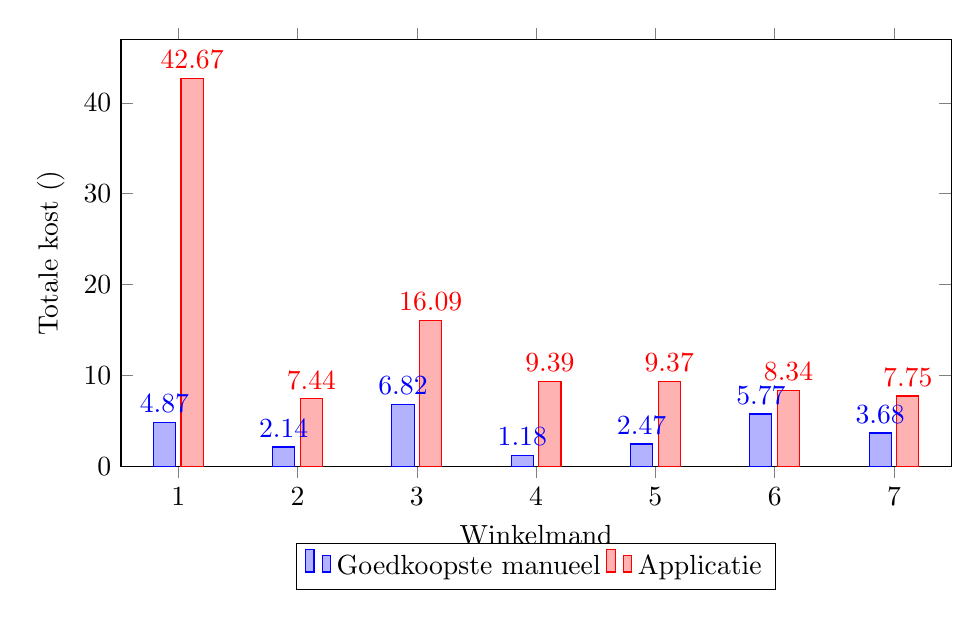
\begin{tikzpicture}
        \begin{axis}[
            ybar,
            bar width=8pt,
            width=\textwidth,
            height=7cm,
            ymin=0,
            ylabel={Totale kost (\euro)},
            xlabel={Winkelmand},
            symbolic x coords={1,2,3,4,5,6,7},
            xtick=data,
            legend style={at={(0.5,-0.18)},anchor=north,legend columns=2},
            nodes near coords,
            nodes near coords align={vertical},
            enlarge x limits=0.08
            ]
            \addplot coordinates {(1,4.87) (2,2.14) (3,6.82) (4,1.18) (5,2.47) (6,5.77) (7,3.68)};
            \addplot coordinates {(1,42.67) (2,7.44) (3,16.09) (4,9.39) (5,9.37) (6,8.34) (7,7.75)};
            \legend{Goedkoopste manueel, Applicatie}
        \end{axis}
    \end{tikzpicture}
    \caption{Vergelijking totale kost: goedkoopste manuele winkel vs.\ applicatie (€/product)}
    \label{fig:bar_costs}
\end{figure}

\subsection{Besparing per winkelmand}
Figuur~\ref{fig:bar_savings} visualiseert de besparing zoals gedefinieerd in Tabel~\ref{tab:savings_price}. Negatieve waarden duiden op een meerkost voor de applicatie.

\begin{figure}[H]
    \centering
    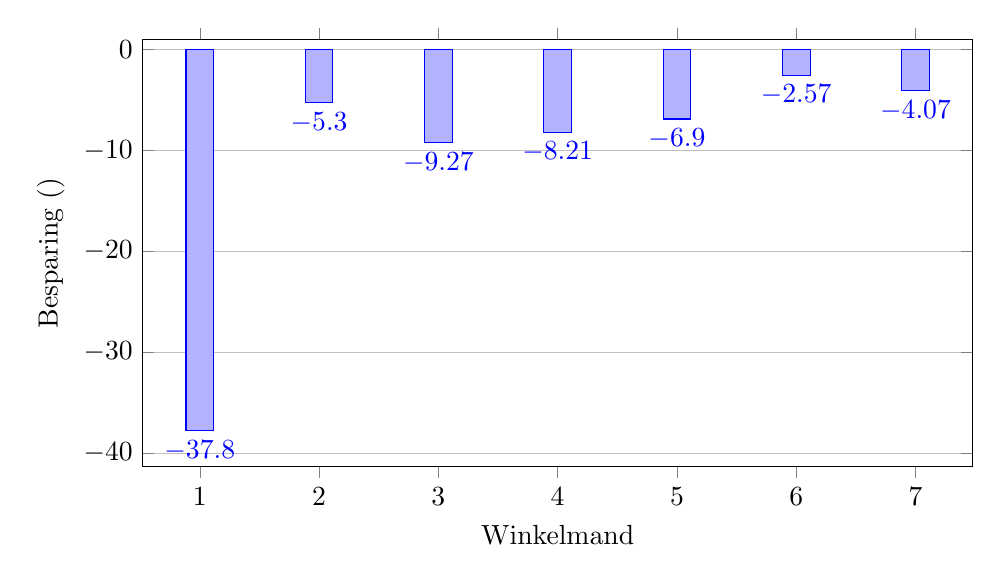
\begin{tikzpicture}
        \begin{axis}[
            ybar,
            bar width=10pt,
            width=\textwidth,
            height=7cm,
            ymajorgrids=true,
            ylabel={Besparing (\euro)},
            xlabel={Winkelmand},
            symbolic x coords={1,2,3,4,5,6,7},
            xtick=data,
            nodes near coords,
            nodes near coords align={vertical},
            enlarge x limits=0.08
            ]
            \addplot coordinates {(1,-37.80) (2,-5.30) (3,-9.27) (4,-8.21) (5,-6.90) (6,-2.57) (7,-4.07)};
        \end{axis}
    \end{tikzpicture}
    \caption{Besparing t.o.v.\ goedkoopste manuele winkel (negatief = applicatie duurder)}
    \label{fig:bar_savings}
\end{figure}

\subsection{Tijdsbesparing}
\label{sec:time}
\begin{table}[H]
    \centering
    \caption{Vergelijking tijdsinvestering}
    \begin{tabular}{lc}
        \toprule
        \textbf{Methode} & \textbf{Gemiddelde tijd} \\
        \midrule
        Manuele vergelijking & 15--25 minuten \\
        Applicatie & $<$ 1 minuut \\
        \bottomrule
    \end{tabular}
    \label{tab:time_comparison}
\end{table}

De applicatie reduceert de benodigde tijd met meer dan 90\% ten opzichte van manuele vergelijking, doordat zoeken, filteren, en het interpreteren van prijs per eenheid geautomatiseerd worden.

\section{Conclusie}
De testresultaten tonen dat de applicatie een sterke meerwaarde biedt op het vlak van snelheid en gebruiksgemak. In deze dataset blijkt de applicatie echter niet goedkoper te zijn dan de goedkoopste manuele winkel in absolute aankoopkost. Dit wijst erop dat de huidige implementatie in sterke mate beïnvloed wordt door semantische mismatches en de keuze van het optimalisatiecriterium (prijs per eenheid versus totale prijs).

Als proof-of-concept bevestigt dit hoofdstuk de technische haalbaarheid en de praktische winst in tijd, en tegelijkertijd duidelijke verbeterpunten aantoont: expliciete productcategorieën, betere semantische filtering, en eventueel een tweede optimalisatiemodus gericht op \emph{laagste totale kost} zijn een must.
